% Mittagessen für die Kalorien-Aufgabe in Kapitel 6 (K06_Datenstrukturen.tex):
% Getränkedose, Sandwich und die beiden Nährwertangaben als TikZ.
% Marken und Produktnamen sind erfunden. Die Werte (26 kcal/100 ml, 33 cl,
% 229 kcal/100 g, 230 g) werden von der Musterlösung kcal_info.py verwendet.
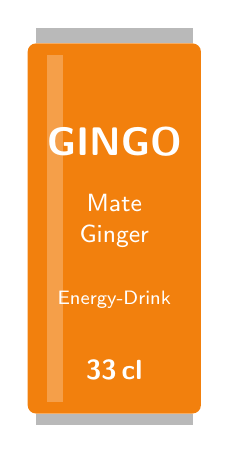
\begin{tikzpicture}[font=\sffamily]
	% Dose (33 cl)
	\fill[orange!80!brown, rounded corners=3pt] (0,0.15) rectangle (2.2,4.85);
	\fill[gray!55] (0.1,4.85) rectangle (2.1,5.05);
	\fill[gray!55] (0.1,0) rectangle (2.1,0.15);
	\fill[white, opacity=.25] (0.25,0.3) rectangle (0.45,4.7);
	\node[white, font=\sffamily\bfseries\Large] at (1.1,3.6) {GINGO};
	\node[white, font=\sffamily\small, align=center] at (1.1,2.6) {Mate\\Ginger};
	\node[white, font=\sffamily\scriptsize] at (1.1,1.6) {Energy-Drink};
	\node[white, font=\sffamily\bfseries] at (1.1,0.7) {33\,cl};
\end{tikzpicture}\hspace{.3cm}%
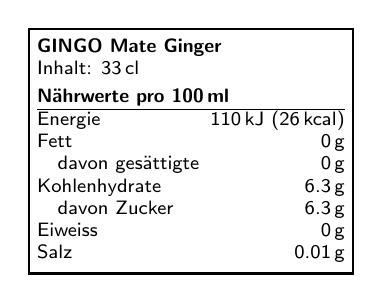
\begin{tikzpicture}[font=\sffamily]
	% Nährwertangabe Getränk
	\node[draw, thick, fill=white, inner sep=3pt, font=\sffamily\scriptsize] {%
		\begin{tabular}{@{}l@{\hspace{4pt}}r@{}}
			\multicolumn{2}{@{}l}{\textbf{GINGO Mate Ginger}}  \\
			\multicolumn{2}{@{}l}{Inhalt: 33\,cl}              \\[2pt]
			\multicolumn{2}{@{}l}{\textbf{Nährwerte pro 100\,ml}} \\
			\hline
			Energie                     & 110\,kJ (26\,kcal)    \\
			Fett                        & 0\,g                  \\
			\quad davon gesättigte      & 0\,g                  \\
			Kohlenhydrate               & 6.3\,g                \\
			\quad davon Zucker          & 6.3\,g                \\
			Eiweiss                     & 0\,g                  \\
			Salz                        & 0.01\,g
		\end{tabular}};
\end{tikzpicture}\hspace{.3cm}%
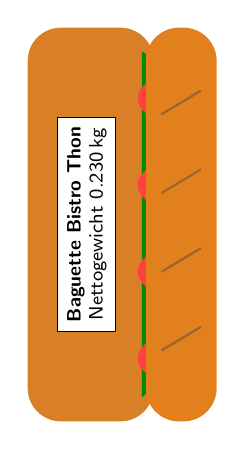
\begin{tikzpicture}[font=\sffamily]
	% Sandwich (Baguette mit Füllung, schräg von der Seite)
	\fill[brown!60!orange, rounded corners=12pt] (0,0) rectangle (1.6,5);
	\fill[green!55!black] (1.45,0.3) -- (1.75,0.6) -- (1.5,0.9) -- (1.75,1.3)
		-- (1.5,1.7) -- (1.75,2.1) -- (1.5,2.5) -- (1.75,2.9) -- (1.5,3.3)
		-- (1.75,3.7) -- (1.5,4.1) -- (1.75,4.5) -- (1.45,4.7) -- cycle;
	\foreach \y in {0.8,1.9,3.0,4.1}{\fill[red!75] (1.62,\y) circle (0.22);}
	\fill[brown!45!orange, rounded corners=12pt] (1.5,0) rectangle (2.4,5);
	\foreach \y in {0.9,1.9,2.9,3.9}{\draw[brown!80!black, thick] (1.7,\y) -- (2.2,\y+0.3);}
	% Etikett
	\node[draw, fill=white, rotate=90, font=\sffamily\scriptsize, align=center]
		at (0.75,2.5) {\textbf{Baguette Bistro Thon}\\Nettogewicht 0.230\,kg};
\end{tikzpicture}\hspace{.3cm}%
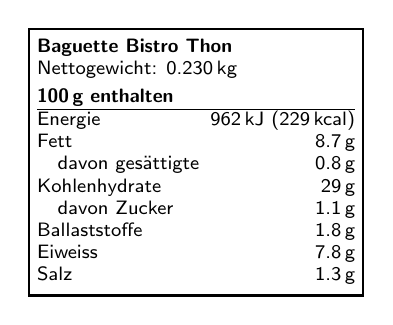
\begin{tikzpicture}[font=\sffamily]
	% Nährwertangabe Sandwich
	\node[draw, thick, fill=white, inner sep=3pt, font=\sffamily\scriptsize] {%
		\begin{tabular}{@{}l@{\hspace{4pt}}r@{}}
			\multicolumn{2}{@{}l}{\textbf{Baguette Bistro Thon}} \\
			\multicolumn{2}{@{}l}{Nettogewicht: 0.230\,kg}      \\[2pt]
			\multicolumn{2}{@{}l}{\textbf{100\,g enthalten}}    \\
			\hline
			Energie                     & 962\,kJ (229\,kcal)   \\
			Fett                        & 8.7\,g                \\
			\quad davon gesättigte      & 0.8\,g                \\
			Kohlenhydrate               & 29\,g                 \\
			\quad davon Zucker          & 1.1\,g                \\
			Ballaststoffe               & 1.8\,g                \\
			Eiweiss                     & 7.8\,g                \\
			Salz                        & 1.3\,g
		\end{tabular}};
\end{tikzpicture}
